\chapter{Practical methods and computational tutorials}\label{ch:11}
\begin{insight}{Learning objectives}
Reproduce an analysis from its data-generating equations; check shapes, units, solver residuals, and stochastic seeds; compare geometric summaries with known ground truth; analyze a complete recurrent state; and design controls that distinguish competing dynamical explanations.
\end{insight}

\section{An executable laboratory for the preceding chapters}
A useful tutorial should let us tell when a method is right, when it is wrong, and when it answers a different question. The nine examples in this chapter therefore use known synthetic systems. The datasets are small enough to inspect and regenerate. Each script saves a vector PDF and a PNG figure, a JSON record of its numerical results, the seed, and package versions. Relevant arrays and the trained network checkpoint are saved as well.

The scripts are independent entry points in the \path{code/} directory and share the small helper \path{common.py}. Python 3.12 was used for the recorded run. The project contains a tested dependency snapshot and a more flexible requirements file. A CPU is sufficient. From the project root:
\begin{lstlisting}[language=bash]
python -m venv .venv
source .venv/bin/activate
python -m pip install -r code/requirements.txt
python code/run_all.py --seed 17
\end{lstlisting}
Individual examples can be run as \path{python code/04_fixed_points.py --seed 17}. Use \path{--out} and \path{--figures} to choose different output directories. The default directories are \path{results/} and \path{figures/} relative to the project. A fixed seed supports repeatability within the recorded software environment; it does not make a statistical conclusion robust to other samples, initializations, or package versions. UMAP's implementation-specific compatibility option is set explicitly when available, and the exact version is recorded \citep{root_umap_docs}.

\subsection{The common data contract}
Unless a script states otherwise, $X\in\R^{n\times p}$ has observations in rows. A trajectory stored as an array has a time axis that must not be silently mixed with independent trial indices. A collection of RNN trials is stored as trials $\times$ time $\times$ hidden units. Plots label the chosen coordinate system. Homology computations use Euclidean distances and $\F_2$ coefficients; a Rips scale is an edge-length threshold. A fixed-point residual is measured in the full model state before projection.

The implementation checks target concrete failure modes. The PCA example checks the known clean rank. The ODE example compares a simulated orbit radius with an analytic value. The fixed-point example verifies analytical Jacobians against finite differences. The RNN example compares an analytical Jacobian with automatic differentiation. These are checks of specified mathematical relationships, not claims that a complex scientific pipeline has been universally validated.

\section{Tutorial 1: three different meanings of dimension}
\subsection{Question, assumptions, and input}
Can a one-dimensional latent variable require two principal components? What happens to an intrinsic-dimension estimate after adding small observation noise? Generate independent angles $\theta_i\sim\operatorname{Uniform}[0,2\pi)$ and an orthonormal matrix $Q\in\R^{24\times2}$, then define
\begin{equation}\label{eq:tutorial-circle}
x_i=Q\begin{bmatrix}\cos\theta_i\\\sin\theta_i\end{bmatrix},
\qquad y_i=x_i+\eta_i,\qquad
\eta_i\sim\mathcal N(0,0.02^2I_{24}).
\end{equation}
There are $n=600$ samples. The clean support is a circle, hence has intrinsic dimension one. Its centered linear span has dimension two with probability one for this sample. The ambient dimension is 24. The noisy distribution has full-dimensional support: a dimension estimate near one would target a noiseless latent model or an intermediate geometric scale, not the literal support of the noisy observations.

\subsection{Algorithm and implementation}
The script computes PCA, participation ratio, and a bias-corrected nearest-neighbor estimate. If $T_j(x)$ is the distance from $x$ to its $j$th nearest other point, use
\begin{equation}
\widehat d_k(x)=\frac{k-2}{\sum_{j=1}^{k-1}\log[T_k(x)/T_j(x)]},\qquad k>2,
\end{equation}
and average the pointwise estimates. The local homogeneous Poisson approximation motivates this correction; finite density gradients, noise, boundaries, and curvature affect it. It is not a universally unbiased estimator \citep{levina2004}. Duplicate observations would produce zero distances and are explicitly rejected.
\lstinputlisting[language=Python,firstline=9,lastline=15,caption={The local dimension estimator in Tutorial 1.}]{code/01_pca_dimension.py}

\subsection{Recorded result and controls}
The clean rank is exactly two and its participation ratio is approximately $1.998$. The clean local estimates remain near one over neighborhood counts $8,16,32,64$. The corresponding noisy estimates are approximately $9.40,6.68,3.43,1.93$. The neighborhood is probing different scales: at very short distances noise occupies many directions; at larger distances the ring structure becomes more influential. The participation ratio changes only modestly, to approximately $2.034$. There is no contradiction: these statistics summarize different properties.

The last panel uses PCA fitted on 400 training rows and reconstruction error on 200 new rows. This error still decreases as retained dimension increases, reaching zero when all 24 directions are kept. Holding out rows alone does not make full-coordinate reconstruction error a valid selector of noiseless rank. A noise-aware likelihood, held-out entries or neurons under an appropriate model, independent repeats, or a prespecified downstream prediction target is needed; see Chapter~\ref{ch:06}.

\begin{figure}[tbp]
\centering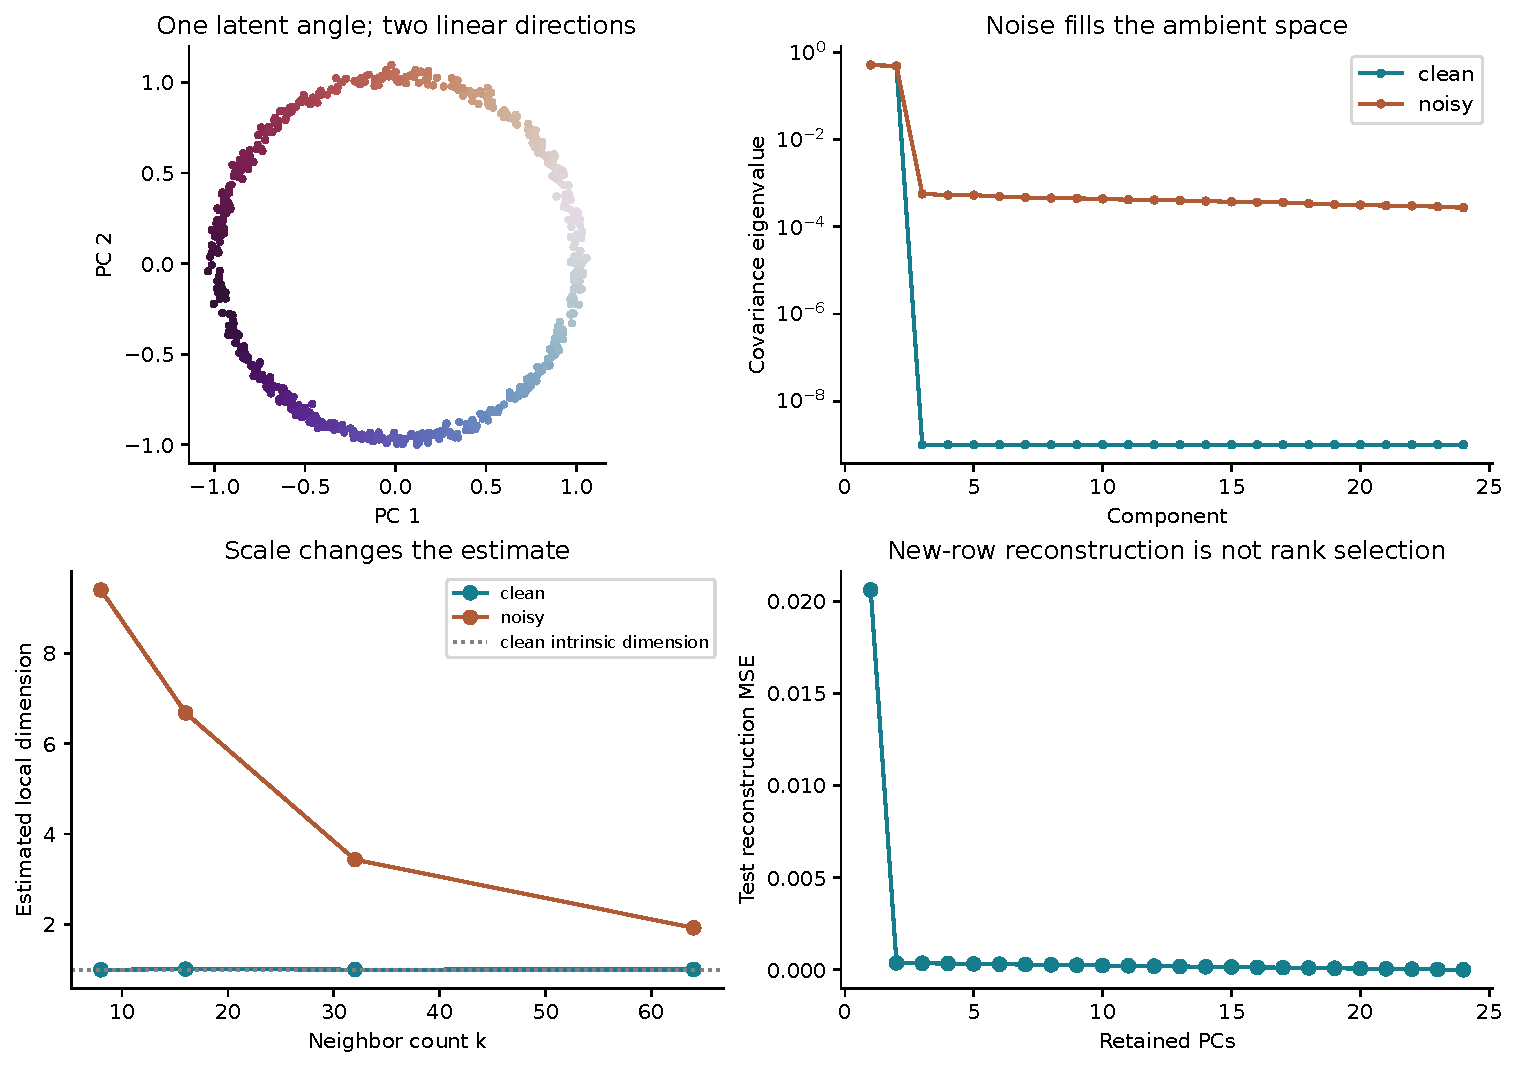
\includegraphics[width=\linewidth]{figures/pca_geometry.pdf}
\caption{Tutorial 1, synthetic data. Color in the upper-left panel denotes the known latent angle. The clean circle has one intrinsic coordinate and two linear directions. The spectra show observation noise beyond the first two components. The lower-left estimates change with neighborhood scale; the lower-right error illustrates why a particular cross-validation target can remain monotone in dimension.}
\label{fig:tutorial-pca}
\end{figure}

Useful controls change noise amplitude, neuron count, sampling density, and the neighborhood range separately. Repeat the clean/noisy comparison after a declared rescaling of each feature. If the estimate changes, identify whether the target metric itself changed. Do not report the smallest estimate as the ``true'' dimension merely because it matches an expectation.

\section{Tutorial 2: comparing embeddings against known geometry}
\subsection{Question and construction}
When does a visually convincing embedding preserve intrinsic distances? A Swiss roll gives a tractable test. Draw $t\in[1.5\pi,4.5\pi]$ and $v\in[0,20]$ independently and uniformly, and map
\begin{equation}
(t,v)\longmapsto(t\cos t,v,t\sin t).
\end{equation}
There are 650 observations with small isotropic coordinate noise. The noiseless induced metric is
\begin{equation}
 ds^2=(1+t^2)\,dt^2+dv^2.
\end{equation}
Set $s(t)=\tfrac12[t\sqrt{1+t^2}+\operatorname{arsinh}(t)]$. Since $ds/dt=\sqrt{1+t^2}$, the coordinates $(s(t),v)$ flatten this rectangular surface isometrically. Their Euclidean distances give an exact ground-truth intrinsic distance for the noiseless surface. Using $t$ directly as a distance coordinate would be wrong.

\subsection{Algorithm and diagnostic quantities}
The script compares PCA, Isomap, and UMAP. Isomap uses a six-neighbor graph for the main display and checks that it is connected. It also runs a twelve-neighbor sensitivity comparison. UMAP uses fifteen neighbors, minimum-distance parameter $0.1$, and a fixed random seed. These settings are transparent demonstration choices, not universal defaults certified for biological recordings.

For sampled pairs, let $a_{ij}$ be intrinsic distance and $b_{ij}$ embedding distance. To remove arbitrary global scale, minimize $\sum_{ij}(c b_{ij}-a_{ij})^2$ over $c$. Differentiation gives
\begin{equation}
 c_* = \frac{\sum a_{ij}b_{ij}}{\sum b_{ij}^2},\qquad
 \operatorname{stress}=\frac{\sqrt{\sum(c_*b_{ij}-a_{ij})^2}}{\sqrt{\sum a_{ij}^2}}.
\end{equation}
Spearman correlation tests the ranking of pairwise distances. Trustworthiness at ten neighbors detects points made spuriously close by the embedding relative to the observed input metric; it does not by itself test intrinsic distance preservation. No single one of these metrics is a complete embedding assessment.

\subsection{Result, parameter sensitivity, and interpretation}
In the recorded example, PCA has scaled intrinsic stress about $0.565$. Six-neighbor Isomap has stress about $0.032$, whereas changing to twelve neighbors raises it to about $0.413$. UMAP has stress about $0.164$. These values characterize this constructed example. They do not establish a general algorithm ranking. A neighborhood graph can remain connected while acquiring harmful shortcuts across different folds; connectivity is a necessary diagnostic here, not a sufficient guarantee of geodesic accuracy.

\begin{figure}[tbp]
\centering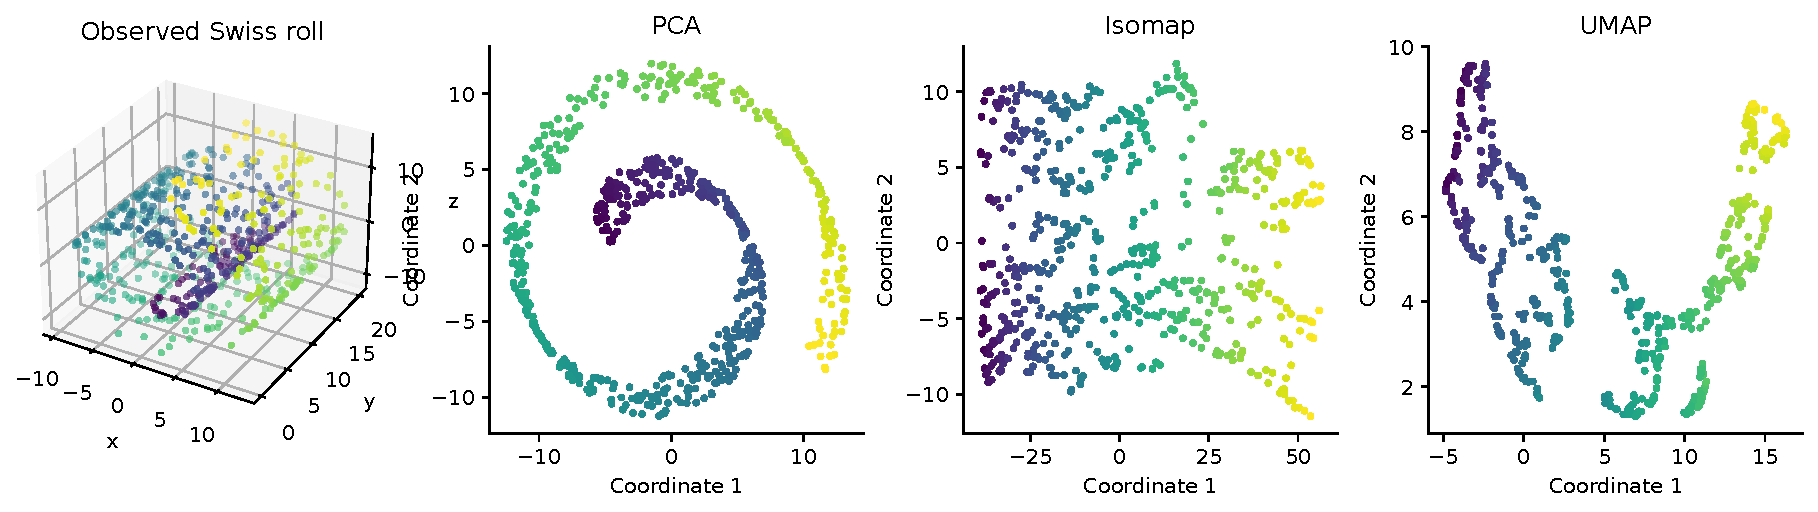
\includegraphics[width=\linewidth]{figures/embeddings.pdf}
\caption{Tutorial 2. All points are colored by the same generating spiral coordinate. PCA, six-neighbor Isomap, and UMAP are fitted to the same noisy Swiss roll. Ground-truth distance metrics and the twelve-neighbor Isomap sensitivity run are saved separately. A pleasing plot and a good local-neighborhood score do not certify global geometry.}
\label{fig:tutorial-embeddings}
\end{figure}

Because ground truth is available, the example can diagnose parameter sensitivity directly. Real experiments usually cannot tune against exact intrinsic distances. They should instead use independent measurements, a defensible generative model, stability across justified parameter ranges, and task-relevant predictions. Trying many settings and reporting only a persuasive ring or cluster is a form of analysis selection.

\section{Tutorial 3: phase portraits and numerical stability}
\subsection{Question, systems, and algorithm}
How do contraction, oscillation, and multiple basins differ? Three two-dimensional systems are simulated with adaptive numerical integration: a stable spiral, the Hopf normal-form oscillator, and a separable double well. The oscillator is
\begin{align}
\dot x&=(\mu-x^2-y^2)x-\omega y,\\
\dot y&=\omega x+(\mu-x^2-y^2)y.
\end{align}
The script compares $\mu=-0.3$ and $\mu=0.8$ with $\omega=1$. The double well uses $\dot x=x-x^3$, $\dot y=-2y$. These are dimensionless demonstration coordinates; they are not measured neural rates.

\lstinputlisting[language=Python,firstline=8,lastline=17,caption={The vector fields used for the phase-portrait examples.}]{code/03_phase_portraits.py}

\subsection{Expected and checked results}
For $\mu>0$, polar coordinates give $\dot r=\mu r-r^3$, so the stable cycle radius is $\sqrt{0.8}\simeq0.894427$. The largest final radius error among the simulated trajectories is below $10^{-8}$ in the recorded run. This comparison checks integration of a known solution property. The double-well trajectories approach either $(1,0)$ or $(-1,0)$ according to the sign of their initial $x$, while the separating stable manifold $x=0$ approaches the saddle at the origin.

\begin{figure}[tbp]
\centering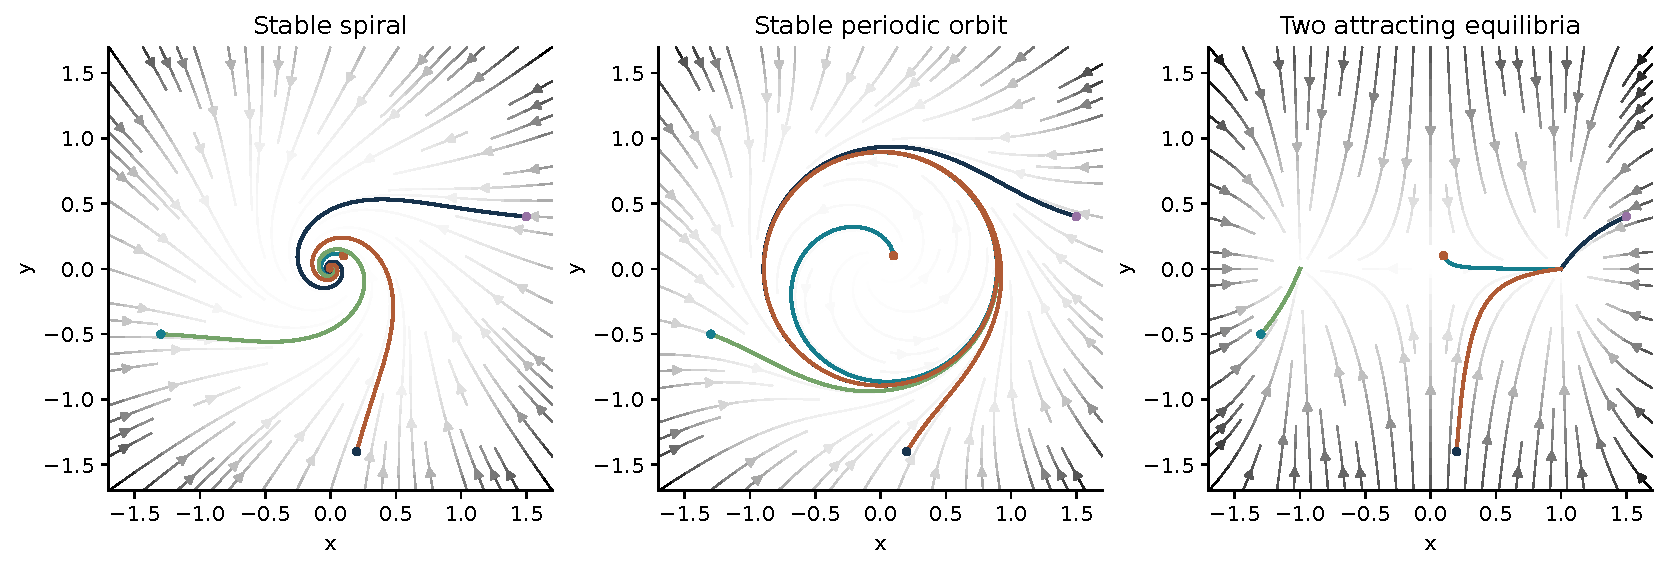
\includegraphics[width=\linewidth]{figures/phase_portraits.pdf}
\caption{Tutorial 3. Gray streamlines depict each vector field; colored curves are trajectories with marked initial states. A sink, a stable periodic orbit, and two attracting equilibria generate distinct phase portraits. Their appearances depend on retaining enough state variables.}
\label{fig:tutorial-phase}
\end{figure}

An additional sanity check contrasts exact evolution and Euler integration for $\dot x=-5x$ with step $\Delta t=0.5$. The exact multiplier is $e^{-2.5}\simeq0.0821$, whereas Euler gives $1-5\Delta t=-1.5$. Thus a numerically growing oscillation can be created by an unstable integration rule applied to a stable ODE. Reduce steps and compare methods before interpreting unexpected divergence. For an SDE, add noise with scale $\sqrt{\Delta t}$, not $\Delta t$; see Chapter~\ref{ch:02} and Appendix~\ref{app:d}.

\section{Tutorial 4: fixed points, residuals, and Jacobians}
\subsection{Question and mathematical model}
Does finding a near-stationary state establish stability? Consider
\begin{equation}
\dot h=-h+W\tanh h,\qquad
W=\diag(1.5,0.7),\qquad h\in\R^2.
\end{equation}
The activation acts before the recurrent matrix in this example. Consequently
\begin{equation}
J(h)=-I+W\diag(1-\tanh^2 h).
\end{equation}
This ordering differs from the equally legitimate model $\dot h=-h+\tanh(Wh)$; copying a Jacobian across the two conventions would be an error.

\subsection{Algorithm and results}
The script starts a numerical root solver from 70 states, checks $\norm{f(h_*)}<10^{-9}$, and merges candidates within $10^{-5}$. It finds approximately $(-1.287839,0)$, $(0,0)$, and $(1.287839,0)$. At the outer roots, the Jacobian eigenvalues are approximately $-0.605687$ and $-0.3$. At the origin they are $0.5$ and $-0.3$. The outer states are locally asymptotically stable; the origin is a saddle.

An independent central-difference calculation checks the analytical Jacobian. With $e_j$ a standard coordinate vector,
\begin{equation}
J_{\cdot j}(h)\approx\frac{f(h+\delta e_j)-f(h-\delta e_j)}{2\delta},
\qquad \delta=10^{-6}.
\end{equation}
Agreement to a declared tolerance detects indexing and derivative mistakes. It does not prove a model is scientifically appropriate.

\begin{figure}[tbp]
\centering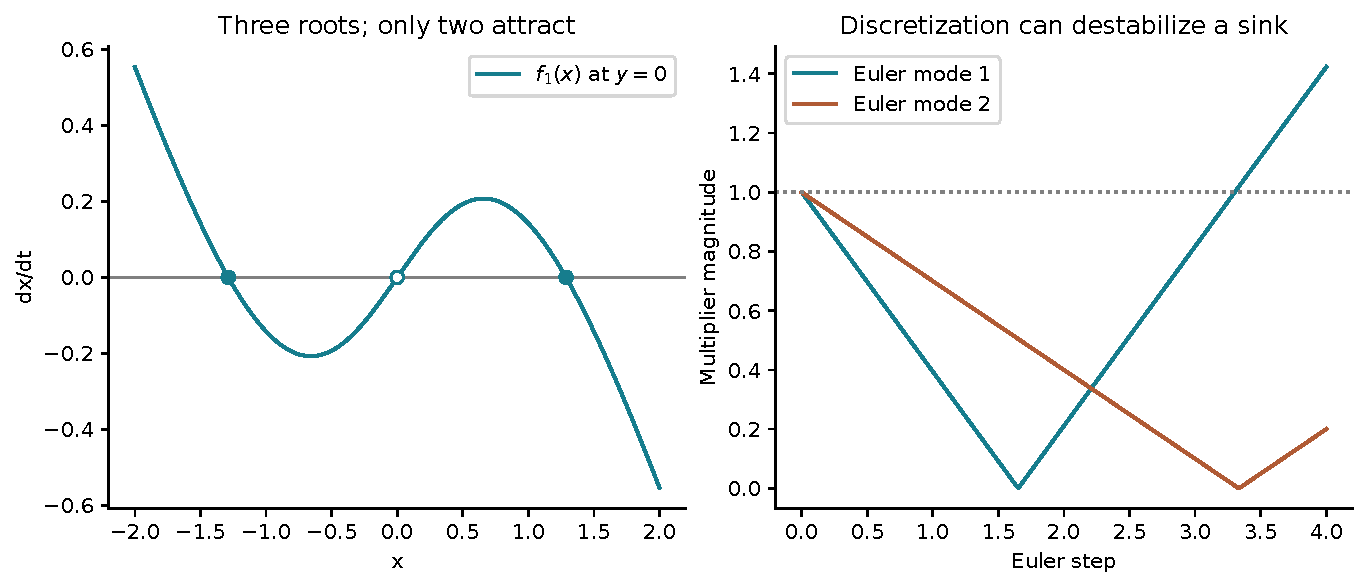
\includegraphics[width=0.96\linewidth]{figures/fixed_points.pdf}
\caption{Tutorial 4. Filled roots are stable in the continuous model and the unfilled root is unstable. The right panel shows magnitudes of the Euler multipliers at an outer equilibrium. Increasing the numerical step eventually destabilizes the discrete approximation even though the ODE remains stable.}
\end{figure}

Multistart search cannot certify that every root has been found. In this particular separable example, additional analytic reasoning can establish the count, but the generic search procedure does not do so. For trained networks, report initialization coverage, residual distributions, deduplication tolerances, and input conditions. Root stability is local; basin size requires further perturbations.

\section{Tutorial 5: a finite ring network and two kinds of perturbation}
\subsection{Question and construction}
What distinguishes attraction toward a family of states from attraction toward one particular state? Place $N=96$ model neurons at preferred angles $\theta_i=2\pi i/N$ and define
\begin{equation}\label{eq:tutorial-ring-rate}
\tau\dot r_i=-r_i+\sigma\!\left(\sum_j W_{ij}r_j\right),\quad
W_{ij}=\frac{-4+14\cos(\theta_i-\theta_j)}{N},\quad
\sigma(a)=\frac{1}{1+e^{-a}},\quad\tau=0.1\,\mathrm{s}.
\end{equation}
Rates are dimensionless and bounded. Euler integration uses $\Delta t=0.002\,\mathrm{s}$. A localized initial activity pattern relaxes to a stationary bump. The example probes an intentionally structured circuit; it does not learn this connectivity from neural data.

\subsection{Algorithm and perturbations}
First equilibrate the network, then restart from the same state for two interventions. At $3\,\mathrm{s}$, the radial intervention replaces $r$ with $0.6r+0.4\bar r\mathbf1$, reducing bump contrast. The phase intervention circularly shifts neuron rates by twelve indices. Track the complex first harmonic
\begin{equation}
 m(t)=\frac1N\sum_j r_j(t)e^{i\theta_j}.
\end{equation}
Its magnitude measures bump contrast and its argument measures phase when the magnitude is nonzero. A low magnitude would make phase estimates ill-conditioned.

The linearization is
\begin{equation}
J=\tau^{-1}\left[-I+\diag\{\sigma'(Wr_*)\}W\right].
\end{equation}
The recorded dimensionless stationary-map residual $\norm{-r_*+\sigma(Wr_*)}$ is below $2\times10^{-14}$; the ODE velocity residual is this quantity divided by $\tau$. The leading numerical eigenvalue is indistinguishable from zero at ordinary floating-point precision, while the next is approximately $-4.844\,\mathrm{s}^{-1}$. This indicates near-neutral phase motion and rapid contraction in another direction in this model.

\begin{figure}[tbp]
\centering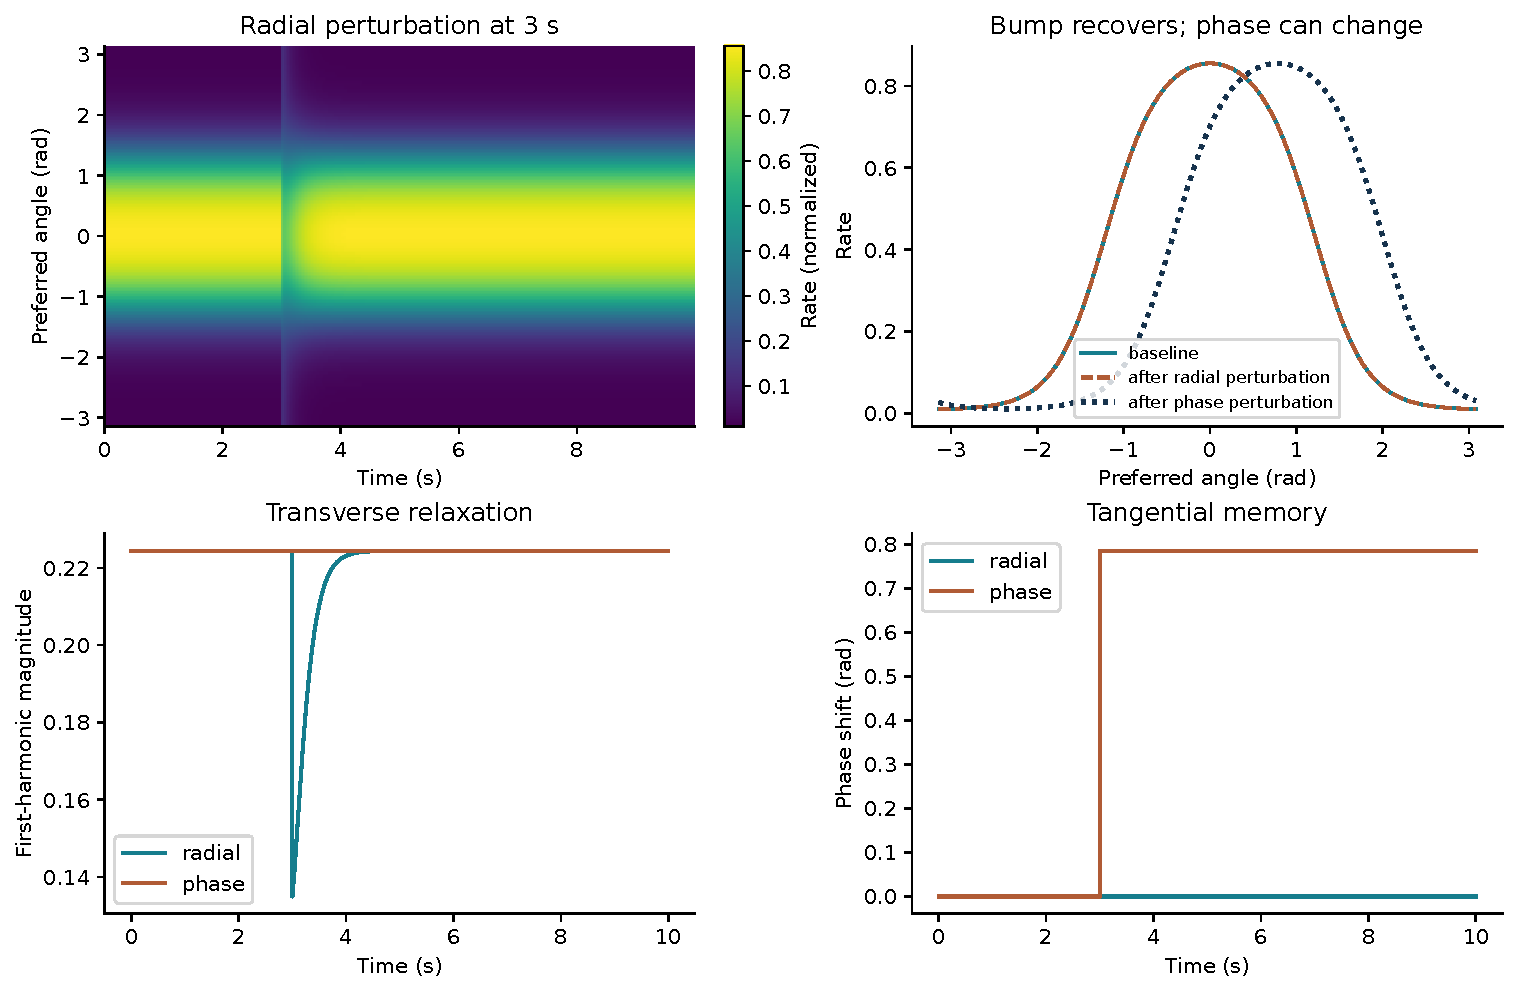
\includegraphics[width=\linewidth]{figures/ring_attractor.pdf}
\caption{Tutorial 5. The heat map and rate profiles show a localized bump. Reducing its contrast is followed by recovery. A phase shift remains, approximately $\pi/4$ for the twelve-neuron shift. The magnitude and phase panels separate transverse relaxation from motion along the represented family.}
\label{fig:tutorial-ring}
\end{figure}

\subsection{Interpretation and limits}
The finite network has exact discrete rotation symmetry, not exact symmetry under every real-valued angle. Very weak pinning can therefore be present even when a computed eigenvalue is nearly zero. Report the numerical tolerance and observation duration. Add heterogeneity, noise, or longer simulations to test robustness. A ring-shaped cloud alone could not establish the transverse relaxation seen in the intervention. Conversely, returning after the radial perturbation does not establish that phase is restored: the phase shift shows why set attraction and point attraction must be distinguished.

\section{Tutorial 6: a circle, sphere, torus, and disk}
\subsection{Question and data}
Can the same pipeline distinguish a prominent loop from a surface cycle, while revealing short-lived holes in a control? The script generates a noisy circle in $\R^2$, a sphere in $\R^3$, a product torus in $\R^4$, and points uniformly distributed across a filled disk. The torus uses
\begin{equation}
(\alpha,\beta)\longmapsto
(\cos\alpha,\sin\alpha,\cos\beta,\sin\beta),
\end{equation}
with a perturbed $14\times14$ angular grid. This is an embedded flat torus. It is different metrically from a doughnut surface in $\R^3$, although both have topology $T^2$. The sphere is generated by normalizing independent Gaussian vectors, which yields uniform directions before noise is added. Disk radii use $r=\sqrt U$ with $U$ uniform; choosing radius uniformly would oversample the center relative to area.

\subsection{Computation and interpretation}
Ripser computes $H_0$, $H_1$, and $H_2$ over $\F_2$ up to maximum edge length $2.3$ \citep{root_ripser}. The noiseless topological targets are $(\beta_0,\beta_1,\beta_2)=(1,1,0)$ for a circle, $(1,0,1)$ for a sphere, $(1,2,1)$ for a torus, and $(1,0,0)$ for a disk. A finite Rips filtration need not display these values at every scale. The diagram records classes of its complexes, not a direct certificate of the continuum object's identity.

\begin{figure}[tbp]
\centering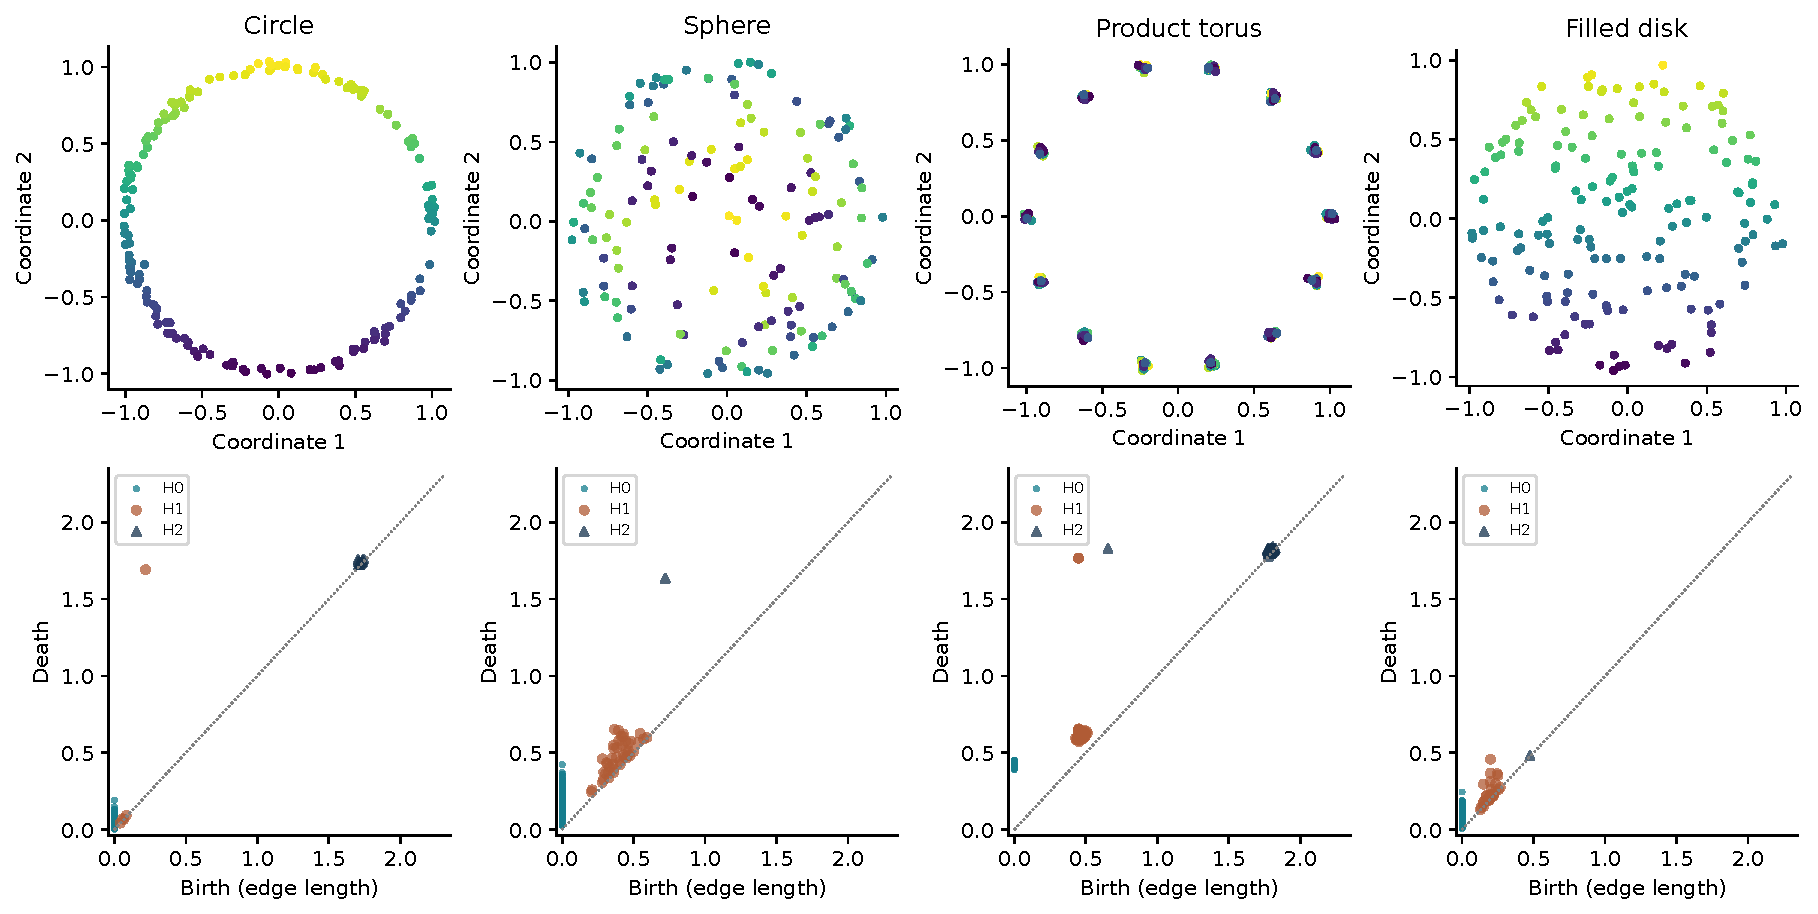
\includegraphics[width=\linewidth]{figures/topology_clouds.pdf}
\caption{Tutorial 6. The upper row shows only the first two observation coordinates; persistence is computed in each dataset's full ambient space. In particular, the torus projection discards an entire circular factor. The lower row shows finite persistence pairs for $H_0$ (dots), $H_1$ (circles), and $H_2$ (triangles). The essential $H_0$ class is omitted from the plotted finite pairs and retained in the saved arrays.}
\label{fig:tutorial-clouds}
\end{figure}

The sphere and torus exhibit long-lived $H_2$ features in this run, while the disk has shorter accidental holes. Even the circle can show small higher-dimensional Rips features at larger scales. A Rips complex is not always a faithful triangulation of the underlying manifold. Inspect intervals jointly, specify the scale range, and compare with appropriate noise and sampling controls. An infinite death time in a truncated calculation can mean a feature has not yet died by the last computed scale; do not automatically call it mathematically essential.

\section{Tutorial 7: a complete neural topological pipeline}
\subsection{Question and observation model}
Can coordinated angular tuning produce a statistically distinguishable loop in held-out population activity? For each of 24 model neurons, place a preferred angle $\phi_j$ evenly on the circle and define a measured rate
\begin{equation}
Y_{ij}=2+4\exp\{2[\cos(\theta_i-\phi_j)-1]\}+\eta_{ij},
\quad\eta_{ij}\sim\mathcal N(0,0.15^2).
\end{equation}
These are continuous noisy rate observations, not Poisson spike counts. Angles are sampled independently. Generate 500 training rows and 180 independent test rows. Fit eight-component PCA only on training data and transform the test rows with this frozen transformation. No label or persistence result is used to select the PCA basis.

\subsection{The statistic and the null}
Compute the test Rips diagram in eight PCA coordinates and define the statistic
\begin{equation}
T=\max_{(b,d)\in D_1,\ d<\infty}(d-b),
\end{equation}
with $T=0$ if no finite $H_1$ class exists. This maximum incorporates selection of the most persistent observed loop. The chosen null is independence between neuron columns across identically distributed independent test observations. Independently permute each raw test column, apply the same frozen PCA transformation, and recompute $T$ for 99 surrogates. Under the stated exchangeability null, the plus-one randomization value is
\begin{equation}
\widehat p=\frac{1+\#\{b:T_b\geq T_{\mathrm{observed}}\}}{100}.
\end{equation}
The minimum attainable value is $0.01$, which is not a statement that the true tail probability equals $0.01$. Selecting preprocessing or a statistic after viewing the test result would require nesting that selection in the null procedure or using additional independent data.

\subsection{Executable core}
The following excerpt includes the generating model, held-out preprocessing, and randomization loop. The full script adds figures and saves all arrays.
\lstinputlisting[language=Python,firstline=9,lastline=31,caption={The central steps of the neural persistence tutorial.}]{code/07_neural_persistence.py}

\subsection{Recorded result, checks, and limits}
The observed maximum $H_1$ lifetime is approximately $9.1655$ in PCA coordinates; the longest among the 99 null maxima is approximately $1.3168$, giving the attainable minimum $\widehat p=0.01$. Computing in the original 24-dimensional observation space also yields a long feature, about $8.9816$. These lifetimes have distance units in their respective spaces and are not universal effect sizes.

\begin{figure}[tbp]
\centering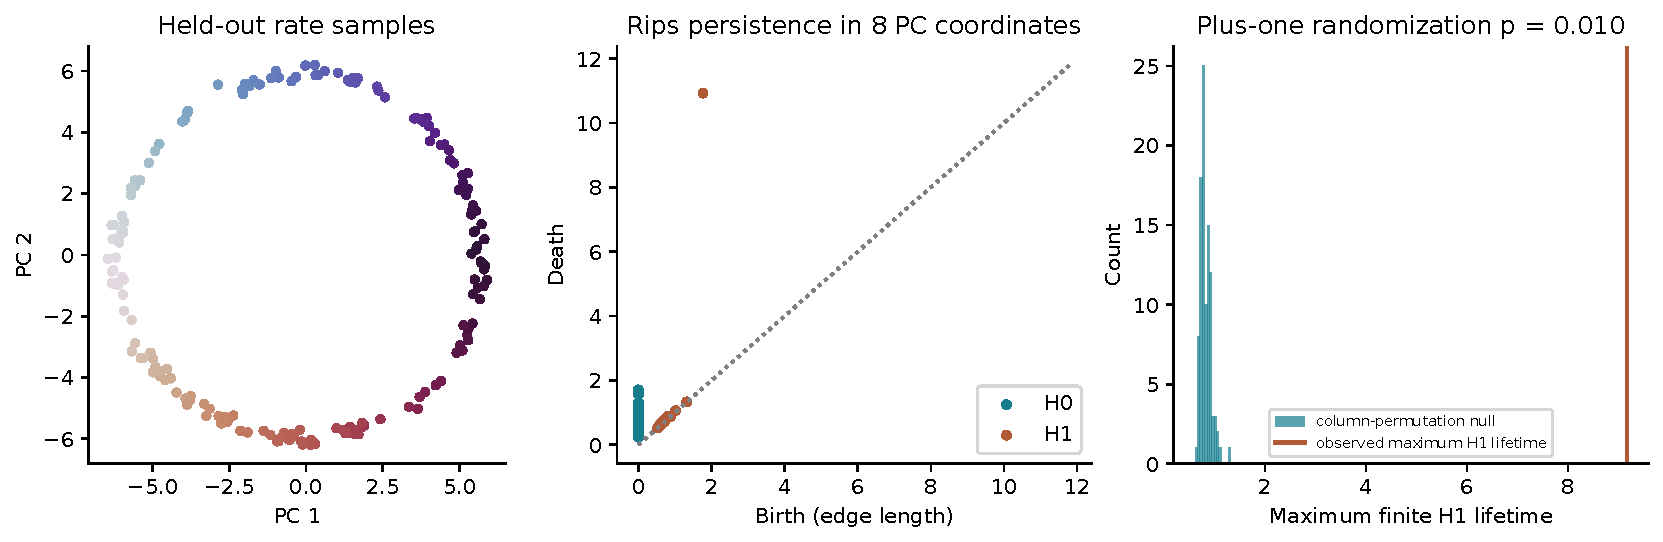
\includegraphics[width=\linewidth]{figures/persistence.pdf}
\caption{Tutorial 7. Left: the first two PCs of held-out observations, colored by generating angle. Middle: the persistence diagram computed using all eight retained PCs. Right: the null distribution of the prespecified maximum $H_1$ lifetime, with the observed statistic marked separately. The analysis establishes incompatibility with the specified independence null, not proof of a recurrent attractor.}
\label{fig:tutorial-persistence}
\end{figure}

The null destroys coordinated population tuning while preserving each neuron's empirical marginal distribution. It does not preserve a behavioral common input, and therefore cannot distinguish a feedforward angular code from an internally generated ring representation. The sampling is independent by construction. Applying this row-permutation scheme to temporally correlated neural recordings would generally be inappropriate. Trial-wise shuffles, circular time shifts, conditional surrogates, or explicit generative nulls answer different questions and require their own exchangeability or modeling assumptions. Chapter~\ref{ch:09} explains the corresponding experimental pipeline.

\section{Tutorial 8: hidden dynamics of a trained recurrent network}
\subsection{Question, task, and training}
Does a trained network solve delayed binary memory with stable states, or only with finite-duration transients? Train a 16-unit tanh RNN on cues of sign $s\in\{-1,+1\}$. Input is present for the first three steps and zero afterward. Cue strengths vary uniformly from $0.8$ to $1.2$ during training. A linear readout predicts the cue sign during the subsequent delay. The training sequence has 35 steps, minibatches have 64 trials, and Adam performs 650 updates. The loss is mean squared prediction error over delay steps.

The recurrent update is
\begin{equation}
h_{t+1}=\tanh(W_hh_t+W_uu_t+b),\qquad
\widehat s_t=w_o^Th_t+b_o.
\end{equation}
The included PyTorch implementation initializes the recurrent matrix orthogonally, clips gradient norm at one, uses double precision, and records the seed and optimizer state. These are training choices, not biological assumptions. The tested API and recurrent-state conventions are documented by PyTorch \citep{root_torch_rnn,app_torchlstm}.

\subsection{Separating training, projection, and dynamical analysis}
After training, freeze all parameters. Probe independent cue strengths from $0.7$ to $1.3$ for 150 steps. Fit PCA on a separate deterministic bank of training-range probe trajectories and project the test states through that same basis. The projection is descriptive. Roots and eigenvalues are computed in the full 16-dimensional state with input fixed at zero:
\begin{equation}
F(h)=\tanh(W_hh+b),\qquad
F(h_*)-h_*=0,\qquad
DF(h_*)=\diag[1-F(h_*)^2]W_h.
\end{equation}
Local stability requires $\rho(DF)<1$. Here the eigenvalues are dimensionless multipliers per recurrent step, not continuous-time rates.

Root searches start from sampled delay states, random states, and zero. Accepted roots have residual below $10^{-8}$; nearby candidates are merged. The script checks the formula for $DF$ against automatic differentiation. For GRUs and LSTMs, the companion utility uses the actual cell implementation, including all gating derivatives. An LSTM state is the concatenation $(h,c)$:
\lstinputlisting[language=Python,firstline=10,lastline=24,caption={Automatic differentiation of the complete recurrent state.}]{code/recurrent_tools.py}
A hidden-only LSTM Jacobian would omit dynamically relevant cell-state directions. The script validates full-state dimensions for a small GRU and LSTM, but the trained demonstration is a tanh RNN; it does not claim to have trained all three architectures.

\subsection{Recorded result and evidential scope}
The recorded seed achieves $100\%$ cue-sign accuracy at step 35 on the test bank. Its mean squared readout error is approximately $1.79\times10^{-8}$ at both steps 35 and 150. The search finds two locally stable roots with spectral radii approximately $0.6211$ and $0.5231$, whose readouts are near $-1$ and $+1$, plus an unstable root with spectral radius approximately $1.7448$. These results support a bistable memory account for this trained instance under zero input.

\begin{figure}[tbp]
\centering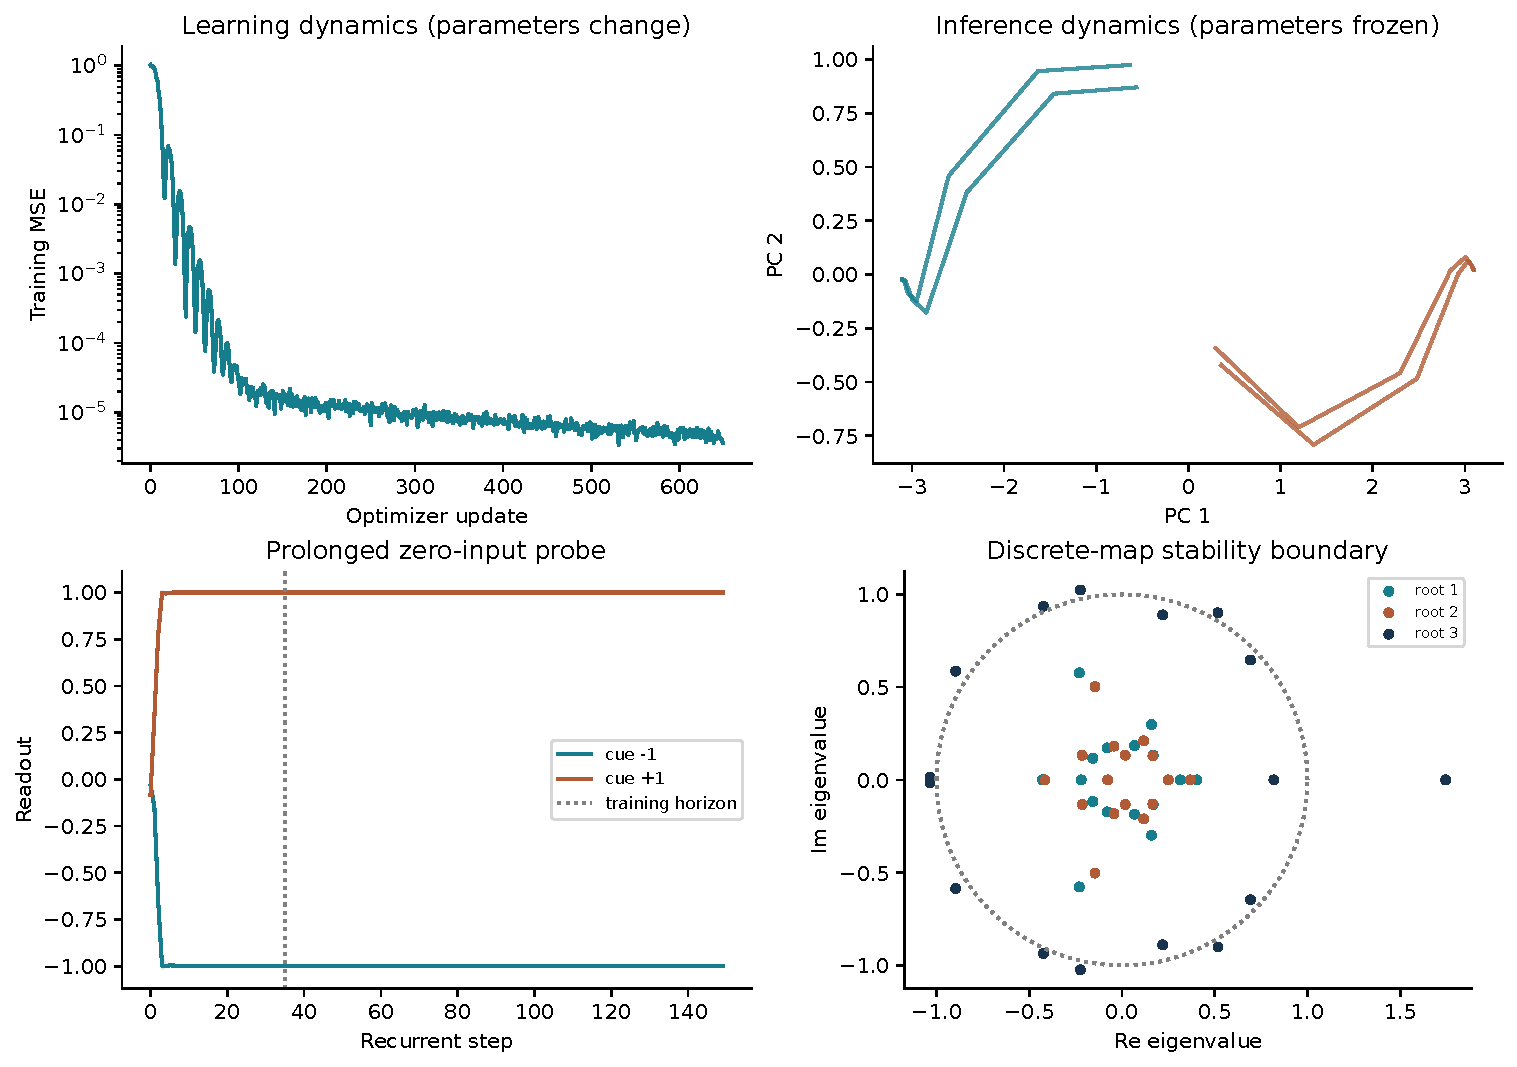
\includegraphics[width=\linewidth]{figures/rnn_dynamics.pdf}
\caption{Tutorial 8. Training loss indexes optimizer updates; hidden trajectories index inference steps after parameters have been frozen. Blue and orange trajectories represent negative and positive cues. The prolonged-delay readout extends beyond the training horizon. The eigenvalue plot compares roots with the discrete-time unit circle; the search is not certified globally complete.}
\label{fig:tutorial-rnn}
\end{figure}

A stronger mechanistic analysis would perturb each candidate root along multiple directions, map basin changes as inputs vary, repeat training across seeds, and test whether the readout uses the predicted state coordinates. The current root search cannot establish that no other equilibria or recurrent structures exist. Successful delayed memory in a different RNN could be transient, input-supported, or distributed across more complicated structures. The checkpoint and probe arrays permit those extensions without retraining this example.

\section{Tutorial 9: identical observations, different mechanisms}
\subsection{A controlled nonidentifiability example}
Suppose the recorded trajectory is exactly $x_0(t)=(\cos t,\sin t)$. Compare two systems:
\begin{align}
\text{Recurrent:}\quad\dot x&=(1-\norm{x}^2)x+Rx,
& R&=\begin{bmatrix}0&-1\\1&0\end{bmatrix},\\
\text{Externally driven:}\quad\dot x&=(-\sin t,\cos t).
\end{align}
Both start at $(1,0)$. The recurrent system has transverse radial contraction toward its unit limit cycle. The second integrates a supplied clock-dependent velocity; its current state does not regulate that velocity. Their unperturbed trajectories, PCA plots, and point-cloud topology coincide. A topology calculation alone therefore cannot distinguish them.

\subsection{Intervention and explicit hypothesis test}
Add the same radial displacement $\delta=0.3$ at the start of each system. In the recurrent system, $\dot r=(1-r^2)r$ restores radius one. In the driven system, the displacement persists as a constant vector offset from the reference path. After one full cycle, compare the signed radial displacement $\norm{x}-1$. Add independent Gaussian observation noise with coordinate standard deviation $0.03$ to 200 repeated observations per model. The prespecified statistic is the difference of group mean radial displacements. A 999-permutation comparison tests equality of the two observation distributions under exchangeability.

\begin{figure}[tbp]
\centering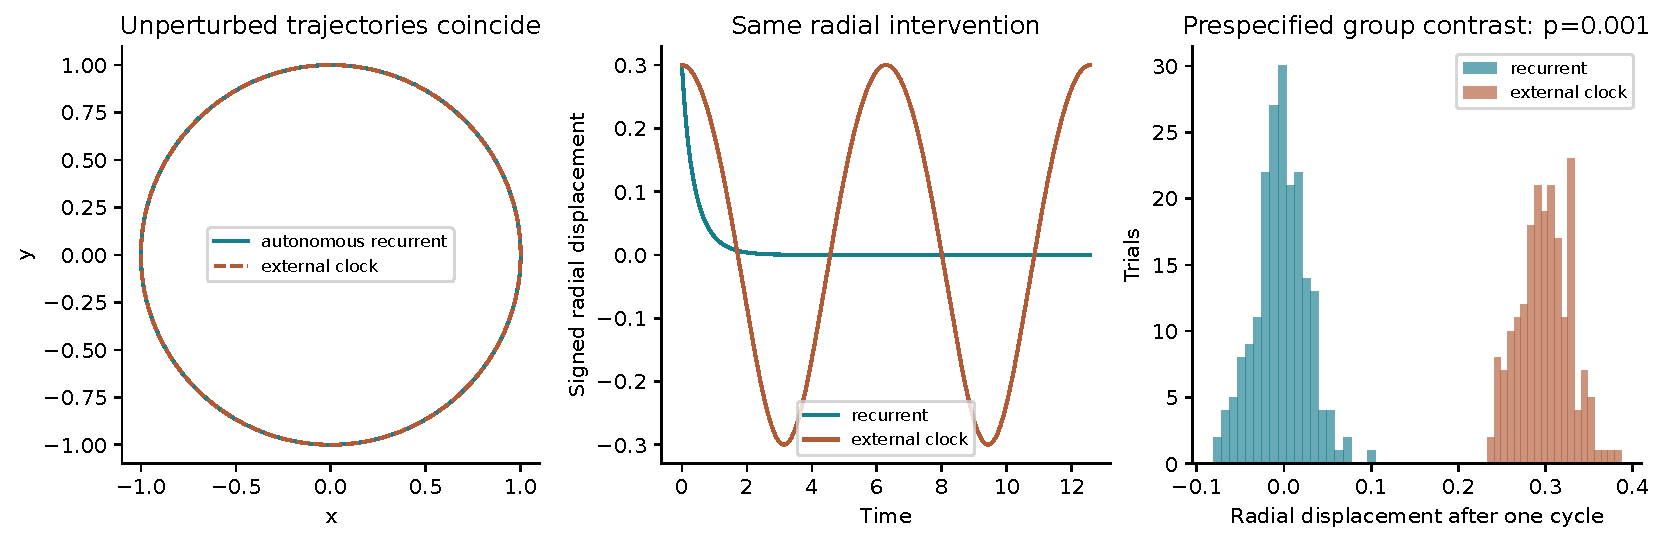
\includegraphics[width=\linewidth]{figures/null_hypotheses.pdf}
\caption{Tutorial 9. The unperturbed trajectories agree to numerical integration precision. A matched radial intervention separates the models. The last panel shows repeated noisy measurements after one complete cycle. The permutation test concerns this declared intervention contrast, not the probability that a model is true.}
\label{fig:tutorial-null}
\end{figure}

The unperturbed numerical discrepancy is below $2\times10^{-10}$ in the recorded run. The intervention mean contrast is about $0.302$ and the plus-one permutation value is $0.001$, the smallest attainable with 999 surrogates. This distinguishes these two specified mechanisms. An externally driven system with feedback could also restore perturbations, so the result would not isolate an entirely internal biological generator without measuring or manipulating the relevant inputs. Chapter~\ref{ch:12} expands this identifiability argument.

\section{What to report when transferring these tools to real data}
A reproducible report should identify the sampling unit, trial structure, preprocessing fitted on each split, observation metric, model state, input condition, estimator, and uncertainty target. For topology, include coefficient field, filtration convention, scale truncation, landmark selection if any, and the statistic used in the null comparison. For dynamics, include time units, differentiation or integration method, fixed-point residuals, Jacobian convention, search initialization, and perturbation sizes. The question is whether another analyst could reproduce both the result and the inference made from it.

There is no single validation protocol that covers every claim. A latent model used to predict firing rates needs held-out prediction assessment. A proposed circular representation needs evidence for periodic structure and appropriate topological or decoding controls. A proposed attractor needs evidence for dynamics toward an invariant set under declared input conditions. A proposed mechanism needs discriminating predictions or interventions. Matching the validation to the claim is the main lesson shared by the tutorials.

\section{Exercises}
\begin{enumerate}
\item \textbf{Introductory.} In Tutorial 1, remove observation noise. Explain why retaining two PCs reconstructs the data exactly although intrinsic dimension is one.
\item \textbf{Introductory.} For Tutorial 4, compute the discrete Euler multipliers at step $\Delta t=4$. Explain why the resulting numerical instability does not change the ODE's local stability.
\item \textbf{Intermediate.} Repeat Tutorial 2 with several neighborhood counts. Record graph connectivity, intrinsic stress, and local trustworthiness before looking at the plots. Can two metrics disagree?
\item \textbf{Intermediate.} Replace the twelve-neuron phase shift in Tutorial 5 with interpolation by half a neuron. Test long-duration drift and explain how finite sampling breaks an ideal symmetry.
\item \textbf{Intermediate.} In Tutorial 7, replace independent angular samples with a slowly varying trajectory. Explain why individual row permutations become an inadequate temporal null, and specify what a new surrogate should preserve.
\item \textbf{Intermediate.} Verify that collapsing the second circular factor in Tutorial 6's torus projection changes what can be identified from two plotted coordinates.
\item \textbf{Advanced.} Train Tutorial 8 across at least five seeds, with shorter training delays and wider test delays. Compare task accuracy, root spectra, and perturbation return. State how you will handle unsuccessful training runs before seeing results.
\item \textbf{Advanced.} Modify the driven model in Tutorial 9 to add feedback from $x-x_0(t)$. Can it now mimic the recurrent perturbation response? Propose a further intervention that distinguishes the new competing models.
\end{enumerate}

\section{Summary and further reading}
These tutorials connect models, observations, statistics, and discriminating controls. Synthetic results validate the declared examples, not biological mechanisms. For method references, see Chapters~\ref{ch:01}, \ref{ch:04}, \ref{ch:06}, and \ref{ch:10}; consult the cited software documentation for implementation details.
